

\tikzset{every picture/.style={line width=0.75pt}} %set default line width to 0.75pt        

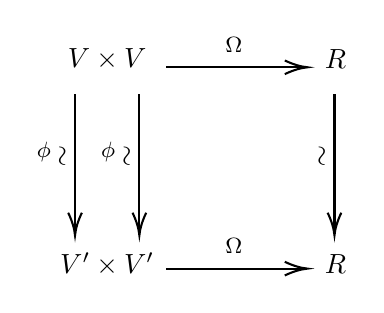
\begin{tikzpicture}[x=0.75pt,y=0.75pt,yscale=-1,xscale=1]
%uncomment if require: \path (0,300); %set diagram left start at 0, and has height of 300

%Straight Lines [id:da494304399766889] 
\draw    (280.5,80) -- (280.5,146) ;
\draw [shift={(280.5,148)}, rotate = 270] [color={rgb, 255:red, 0; green, 0; blue, 0 }  ][line width=0.75]    (10.93,-3.29) .. controls (6.95,-1.4) and (3.31,-0.3) .. (0,0) .. controls (3.31,0.3) and (6.95,1.4) .. (10.93,3.29)   ;
%Straight Lines [id:da03077396523282072] 
\draw    (155.5,80) -- (155.5,146) ;
\draw [shift={(155.5,148)}, rotate = 270] [color={rgb, 255:red, 0; green, 0; blue, 0 }  ][line width=0.75]    (10.93,-3.29) .. controls (6.95,-1.4) and (3.31,-0.3) .. (0,0) .. controls (3.31,0.3) and (6.95,1.4) .. (10.93,3.29)   ;
%Straight Lines [id:da8293026809275621] 
\draw    (186.5,80) -- (186.5,146) ;
\draw [shift={(186.5,148)}, rotate = 270] [color={rgb, 255:red, 0; green, 0; blue, 0 }  ][line width=0.75]    (10.93,-3.29) .. controls (6.95,-1.4) and (3.31,-0.3) .. (0,0) .. controls (3.31,0.3) and (6.95,1.4) .. (10.93,3.29)   ;
%Straight Lines [id:da4027318316111741] 
\draw    (199.5,67) -- (265.5,67) ;
\draw [shift={(267.5,67)}, rotate = 180] [color={rgb, 255:red, 0; green, 0; blue, 0 }  ][line width=0.75]    (10.93,-3.29) .. controls (6.95,-1.4) and (3.31,-0.3) .. (0,0) .. controls (3.31,0.3) and (6.95,1.4) .. (10.93,3.29)   ;
%Straight Lines [id:da5650396736156633] 
\draw    (199.5,164) -- (265.5,164) ;
\draw [shift={(267.5,164)}, rotate = 180] [color={rgb, 255:red, 0; green, 0; blue, 0 }  ][line width=0.75]    (10.93,-3.29) .. controls (6.95,-1.4) and (3.31,-0.3) .. (0,0) .. controls (3.31,0.3) and (6.95,1.4) .. (10.93,3.29)   ;

% Text Node
\draw (171,63) node    {$V\times V$};
% Text Node
\draw (171,162) node    {$V'\times V'$};
% Text Node
\draw (273.5,110) node  [rotate=-90]  {$\sim $};
% Text Node
\draw (148.5,110) node  [rotate=-90]  {$\sim $};
% Text Node
\draw (179.5,110) node  [rotate=-90]  {$\sim $};
% Text Node
\draw (232,56) node  [font=\footnotesize]  {$\Omega $};
% Text Node
\draw (232,153) node  [font=\footnotesize]  {$\Omega $};
% Text Node
\draw (281,63) node    {$\mathbb{R}$};
% Text Node
\draw (281,162) node    {$\mathbb{R}$};
% Text Node
\draw (140.5,108) node  [font=\footnotesize]  {$\phi $};
% Text Node
\draw (171.5,108) node  [font=\footnotesize]  {$\phi $};


\end{tikzpicture}